\section*{Prestazioni dei Sistemi di Comunicazione Numerici in Banda Base}
Nel valutare le prestazioni dei sistemi di comunicazioni numerici in banda base considereremo due fenomeni peggiorativi:
\begin{enumerate}
    \item Interferenza intersimbolo (ISI)
    \item Presenza di rumore
\end{enumerate}

Per il momento ignoriamo il rumore e ci concentriamo sul primo problema.

\subsection*{Interferenza intersimbolica (ISI)}
Il primo fenomeno è causato dalla non perfetta risposta in frequenza del canale di trasmissione e quindi dalle distorsioni lineari introdotte da questo.

\noindent
\begin{minipage}{.5\textwidth}
    \centering
    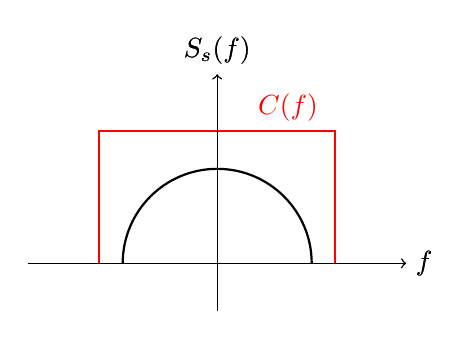
\begin{tikzpicture}[scale=0.6]
        % Canale ideale
        \draw[->] (-1,0) -- (4,0) node[right] {$f$}; % asse x
        \draw[->] (0,-1) -- (0,4) node[above] {$S_s(f)$}; % asse y
        \draw[thick, red] (-2.5,0) -- (-2.5,2.8) -- (2.5,2.8) -- (2.5,0); % rettangolo

        \draw[->] (-4,0) -- (4,0) node[right] {$f$}; % asse x
        \draw[->] (0,-1) -- (0,4) node[above] {$S_s(f)$}; % asse y
        \draw[thick, black] (-2,0) arc (180:0:2);

        \node[red, above] at (1.5,2.8) {$C(f)$};

        % Canale non ideale
        \begin{scope}[shift={(6,0)}] % sposta tutto a destra

        \end{scope}
    \end{tikzpicture}
    \\
    \textbf{Assenza di ISI:}
    \[
        y[k] = f(x[k])
    \]
    \\
\end{minipage}%
\begin{minipage}{.5\textwidth}
    \centering

    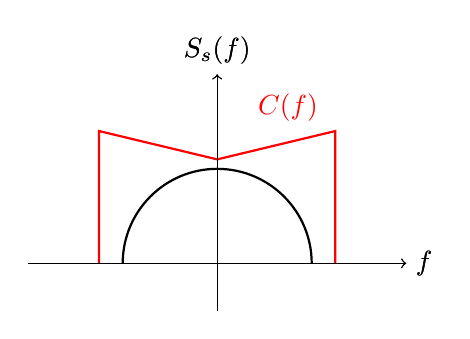
\begin{tikzpicture}[scale=0.6]
        % Canale ideale
        \draw[->] (-1,0) -- (4,0) node[right] {$f$}; % asse x
        \draw[->] (0,-1) -- (0,4) node[above] {$S_s(f)$}; % asse y
        \draw[thick, red] (-2.5,0) -- (-2.5,2.8) -- (0, 2.2) -- (2.5,2.8) -- (2.5,0); % rettangolo

        \draw[->] (-4,0) -- (4,0) node[right] {$f$}; % asse x
        \draw[->] (0,-1) -- (0,4) node[above] {$S_s(f)$}; % asse y
        \draw[thick, black] (-2,0) arc (180:0:2);

        \node[red, above] at (1.5,2.8) {$C(f)$};

        \begin{scope}[shift={(6,0)}] % sposta tutto a destra
        \end{scope}
    \end{tikzpicture}
    \\
    \textbf{Presenza di ISI:}
    \[
        y[k] = f(\dots, x[k-1], x[k], x[k+1], \dots)
    \]
    \\
\end{minipage}


Il risultato è che il campione estratto al ricevitore dal segnale ricevuto al k-esimo istante non dipende solo dal k-esimo simbolo.

\begin{center}
    \begin{tikzpicture}[
            block/.style={rectangle, draw, minimum height=1cm, minimum width=2.5cm},
            node distance=1cm and 2cm,
            auto
        ]

        \node[block] (filter) {$h_R(t)$};
        \node[left=of filter] (channel) {};
        \node[right=of filter] (sampler) {};

        \draw[->] (channel) -- (filter) node[midway,above] {$r(t)$};

        \draw ([xshift=0]filter.east) -- ([xshift=1cm]filter.east) node[midway,above] {$y(t)$};
        \draw ([xshift=1cm]filter.east) -- ([xshift=1.5cm,yshift=0.5cm]filter.east) node[midway,below, yshift=-0.2cm] {$T_s$};

        \draw[->] ([xshift=1.5cm,yshift=0cm]filter.east) -- ++(1.5cm,0) node[midway,above] {$y[n]$};


    \end{tikzpicture}
\end{center}





Per ridurre gli effetti dell'ISI si devono considerare:
\begin{enumerate}
    \item il sagomatore in trasmissione \( p(t) \)
    \item la risposta impulsiva del canale \( c(t) \)
    \item il filtro in ricezione
\end{enumerate}

\begin{center}
    \begin{tikzpicture}[
            block/.style={rectangle, draw, minimum height=1cm, minimum width=2.5cm},
            node distance=1cm and 2cm,
            auto
        ]
        \node[block] (interpolatore) {$p(t)$};
        \node[left=of interpolatore] (tmp) {};
        \node[block, right= of interpolatore] (chan) {$c(t)$};
        \node[block, right= of chan] (filter) {$h_R(t)$};
        \node[right=of filter] (sampler) {};

        \draw[->] (channel) -- (interpolatore) node[midway,above] {$x[k]$};
        \draw[->] (interpolatore) -- (chan) node[midway,above] {$s(t)$};
        \draw[->] (chan) -- (filter) node[midway,above] {$r(t)$};

        \draw ([xshift=0]filter.east) -- ([xshift=1cm]filter.east) node[midway,above] {$y[k]$};
        \draw ([xshift=1cm]filter.east) -- ([xshift=1.5cm,yshift=0.5cm]filter.east) node[midway,below, yshift=-0.2cm] {$T_s$};

        \draw[->] ([xshift=1.5cm,yshift=0cm]filter.east) -- ++(1.5cm,0) node[midway,above] {$y[n]$};

        \draw[dashed, red, thick] ([xshift=-0.5cm,yshift=0.5cm]interpolatore.north west) rectangle ([xshift=0.5cm,yshift=-0.5cm]filter.south east);

        \node[align=center, red, above right= -1cm and -6cm of filter.south east] (channel-label) {$h(t)$};


    \end{tikzpicture}
\end{center}
\[
    h(t)=p(t) \ast c(t) \ast h_R(t)
\]

\paragraph*{Dimostrazione}
\[ Y(f) = R(f) \cdot H_R(f) = S(f) \cdot C(f) \cdot H_R(f) = \overline{X}(f) \cdot P(f) \cdot C(f) \cdot H_R(f) \]
\[ = \overline{X}(f) \cdot H(f) \quad  \text{dove} \quad H(f) = P(f) \cdot C(f) \cdot H_R(f) \]

\[ y(t) = \sum_{n=-\infty}^{+\infty} x[n] \cdot h(t - nT_s) \]

\[ y[k] = y(kT_s) = \sum_{n=-\infty}^{+\infty} x[n] \cdot h((k - n) \cdot T_s)  \]
\[ = x[k] \cdot h(0) + \sum_{\substack{n=-\infty \\ n \neq k}}^{+\infty} x[n]\cdot h((k - n) \cdot T_s) \]

Il secondo termine rappresenta la componente ISI.




\subsection*{Canale con ISI}

Un canale con banda \( B_c \) in generale introduce ISI. Ci sono due aspetti di cui ci occuperemo:

\begin{enumerate}
    \item Determinazione del \( T_s \) minimo che può essere adottato al fine di ottenere una sequenza campionata priva di ISI.
    \item Determinare le condizioni sotto le quali è possibile trasmettere un segnale M-PAM attraverso un canale non ideale in modo che non vi sia ISI nella sequenza campionata.
\end{enumerate}

Nel risolvere i due problemi riterremo \( c(t) \) fissata, e \( p(t) \) e \( h_R(t) \) variabili, in quanto determinabili dal progettista.

Un approccio non perseguibileconsiste nel trasmettere impulsi di durata finita e quindi con banda illimitata. Questo è in contrasto con la limitatezza messa a disposizione dal canale di trasmissione \( (B_c < \infty) \).

\(\Rightarrow\) Gli impulsi \( p(t) \) devono avere durata infinita.

\subsection*{Primo criterio di Nyquist per la trasmissione priva di ISI}

\[ h(kT_s) =
    \begin{cases}
        1, & \text{se } k=0      \\
        0, & \text{se } k \neq 0
    \end{cases}
    \quad \text{(Dominio del tempo)}
\]

\[ \sum_{k=-\infty}^{+\infty} H\left(f-\frac{k}{T_s}\right) = T_s \quad \forall f \quad \text{(Dominio della frequenza)} \]




\paragraph*{Dimostrazione}
Il primo criterio di Nyquist nel dominio del tempo garantisce l'assenza di ISI in quanto
\[ y[k] = x[k] \cdot h(0) + \sum_{\substack{n=-\infty \\ n \neq k}}^{+\infty} x[n] \cdot h((n-k)T_s) = x[k] \cdot h(0) \]
dove il secondo termine è nullo e non vi è ISI se \( h[n] = \delta[n] \).

La relazione in frequenza si ottiene come trasformazione
\[ h[k] = \delta[k] \quad \Longleftrightarrow \quad \overline{H}(f) = 1 \quad \forall f \]
\[ \overline{H}(f) = \frac{1}{T_s} \sum_{k=-\infty}^{+\infty} H\left(f - \frac{k}{T_s}\right) = 1 \quad \forall f \]
\[ \sum_{k=-\infty}^{+\infty} H\left(f - \frac{k}{T_s}\right) = T_s \quad \forall f \]

\subsection*{Trasmissione priva di ISI}
Supponiamo sia assegnato un canale a banda rigorosamente limitata con banda \( B_c \).
\[ C(f) = 0 \quad \text{per} \quad |f| > B_c \]
e supponiamo che \( B_T = B_c \), ovvero che il segnale trasmesso occupa tutta la banda messa a disposizione dal canale.
Allora si verificano le seguenti:
\begin{enumerate}
    \item Non è possibile in alcun modo eliminare l'ISI quando \( T_s < \frac{1}{2B_c} \).


          \paragraph*{Dimostrazione:}

          Quando \( T_s < \frac{1}{2B_c} \)

          \begin{tikzpicture}[scale=0.5]
              \draw[->] (-15,0) -- (15,0) node[right] {\( f \)};
              \draw[->] (0,-1) -- (0,7) node[above] {\( \overline{H}(f) \)};

              % Triangles
              \draw (-11,0) -- (-8,3) -- (-5,0);
              \draw[dashed, red] (-5,-1) -- (-5,4);
              \draw[dashed, red] (-3,-1) -- (-3,4);
              \draw (-3,0) -- (0,3) -- (3,0);
              \draw[dashed, red] (3,-1) -- (3,4);
              \draw[dashed, red] (5,-1) -- (5,4);
              \draw (5,0) -- (8,3) -- (11,0);

              \node at (-12,1.5) {\( \cdots \)};
              \node at (12,1.5) {\( \cdots \)};
          \end{tikzpicture}

          Esistono degli intervalli di frequenza dove \( \overline{H}(f) = 0 \) per cui non può mai accadere che \( \overline{H}(f) = 1 \) \( \forall f \)

          \bigskip

    \item Il più piccolo valore di \( T_s \) che permette di eliminare l'\( ISI \) è

          \( T_s^{(min)} = \frac{1}{2B_c} \)

          \bigskip

          \( f_s^{(max)}\) = \( \frac{1}{T_s^{(min)}} = 2B_c = f_N \) \quad (frequenza di Nyquist)

          \bigskip

          \begin{tikzpicture}[scale=0.5]
              \draw[->] (-15,0) -- (15,0) node[right] {\( f \)};
              \draw[->] (0,-1) -- (0,7) node[above] {\( \overline{H}(f) \)};

              % Triangles
              \draw (-9,0) -- (-6,3) -- (-3,0);
              \draw (-3,0) -- (0,3) -- (3,0);
              \draw (3,0) -- (6,3) -- (9,0);

              \node at (-10,1.5) {\( \cdots \)};
              \node at (10,1.5) {\( \cdots \)};
              \
          \end{tikzpicture}

          Non esistono intervalli di frequenza dove \( \overline{H}(f) = 0 \)

          \bigskip

    \item Nel caso valga la condizione \( T_s = \frac{1}{2B_c} \), allora l'unica funzione di trasferimento che permette di eliminare completamente l'\( ISI \) è

          \[ H(f) = \frac{1}{2B_c} \text{rect}\left(\frac{f}{2B_c}\right) \quad \Leftrightarrow \quad h(t) = \text{sinc}(2B_c t) \]





          \paragraph*{Dimostrazione:}

          \begin{center}

              \begin{tikzpicture}[scale=1]
                  \begin{axis}[
                          axis lines=middle,
                          xlabel={$f$},
                          ylabel={$H(f)$},
                          xtick={-4, -2, 2, 4},
                          xticklabels={$-2B_c$, $-B_c$, $B_c$, $2B_c$},
                          ytick={100},
                          yticklabels={},
                          ymin=-0.2, ymax=2,
                          xmin=-8, xmax=8,
                          %every axis x label/.style={at={(ticklabel* cs:1.05)}, anchor=west,},
                          %every axis y label/.style={at={(ticklabel* cs:1.05)}, anchor=south,},
                          xmajorgrids=false,
                          ymajorgrids=false,
                          clip=false
                      ]

                      % Draw the rectangle
                      \draw [thick] (axis cs:-2,0) rectangle (axis cs:2,0.4);

                      % Add the summation formula
                      \node [red]at (axis cs:7,0.6) {$\sum_{k=-\infty}^{\infty} H(f - \frac{k}{T_s})$};

                      % Draw the dashed lines
                      \draw [dashed, red] (axis cs:-6,0.4) -- (axis cs:-6,0);

                      \draw [dashed, red] (axis cs:-8,0.4) -- (axis cs:-2,0.4);
                      \draw [dashed, red] (axis cs:2,0.4) -- (axis cs:8,0.4);

                      \draw [dashed, red] (axis cs:6,0.4) -- (axis cs:6,0);

                  \end{axis}
                  \
              \end{tikzpicture}
          \end{center}

          Si nota anche che la funzione $\text{sinc}(2Bt)$ si annulla quando $t = \frac{k}{2B}$ con $k \neq 0$ per cui
          \[
              h[kT_s] = \text{sinc} \left(2B_c\cdot\frac{k}{2B_c}\right) = \text{sinc}(k) = \left\{
              \begin{array}{ll}
                  1 & \text{se } k=0    \\
                  0 & \text{se } k\neq0
              \end{array}
              \right.
          \]
\end{enumerate}


\textbf{Limiti di applicabilità della funzione di trasferimento rettangolare:}

\begin{enumerate}
    \item Realizzabilità di una funzione di trasferimento rettangolare: risposte in frequenza ideali come quella rettangolare non sono fisicamente realizzabili (Criterio di Paley-Wiener).
    \item Piccoli errori di campionamento provocano un ISI molto grande poiché la funzione $\text{sinc}(2B_ct)$ decresce molto lentamente.
\end{enumerate}

Un errore è nel campionatore induce un ISI grande in quanto si sommano molte contributi!




\begin{figure}[ht]
    \centering
    \begin{center}
        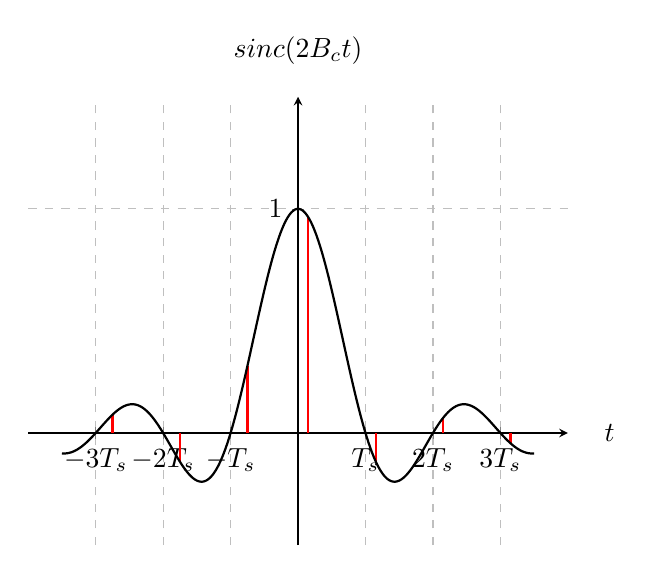
\begin{tikzpicture}
            \begin{axis}[
                    axis lines=middle,
                    xlabel={$t$},
                    ylabel={$\text{sinc}(2B_c t)$},
                    xtick={-3, -2, -1, 0, 1, 2, 3},
                    xticklabels={$-3T_s$, $-2T_s$, $-T_s$, $0$, $T_s$, $2T_s$, $3T_s$},
                    ytick={1},
                    ymin=-0.5, ymax=1.5,
                    xmin=-4, xmax=4,
                    every axis x label/.style={at={(ticklabel* cs:1.05)}, anchor=west,},
                    every axis y label/.style={at={(ticklabel* cs:1.05)}, anchor=south,},
                    xmajorgrids=true,
                    ymajorgrids=true,
                    grid style=dashed,
                    clip=false,
                    no markers,
                    samples=1000,
                    domain=-3.5:3.5
                ]


                \draw [thick, red] (axis cs:-2.75,0) -- (axis cs:-2.75,0.082);
                \draw [thick, red] (axis cs:-1.75,0) -- (axis cs:-1.75,-0.13);
                \draw [thick, red] (axis cs:-0.75,0) -- (axis cs:-0.75,0.30);

                \draw [thick, red] (axis cs:0.15,0) -- (axis cs:0.15,0.965);

                \draw [thick, red] (axis cs:1.15,0) -- (axis cs:1.15,-0.125);
                \draw [thick, red] (axis cs:2.15,0) -- (axis cs:2.15,0.07);
                \draw [thick, red] (axis cs:3.15,0) -- (axis cs:3.15,-0.045);


                % Define sinc function
                \addplot+[thick, black, smooth, unbounded coords=jump] {sin(deg(pi*x))/(pi*x)};
                \addplot+[thick, black, smooth] coordinates {(0, 1)};

                % Add the red vertical line at t=0

            \end{axis}
        \end{tikzpicture}
    \end{center}
    \caption*{Un errore $\epsilon$ nel campionatore induce un ISI grande in quanto si sommano molti contributi. In rosso l'errore $\epsilon$ del compionatore.}
    %\label{fig:my_label} % Optional, for referencing the figure
\end{figure}



Rilassando la condizione $T_s > \frac{1}{2B_c}$, ovvero ammettendo

\[ T_s > \frac{1}{2B_c} \]

si ottiene il seguente effetto:

\begin{center}

    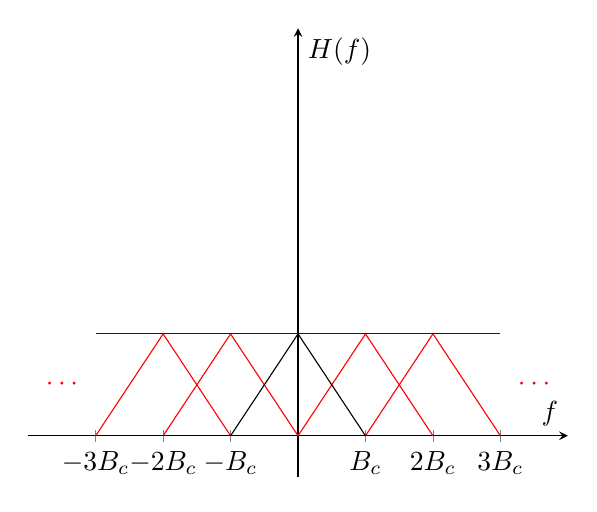
\begin{tikzpicture}[scale=1]
        \begin{axis}[
                axis lines=middle,
                xlabel={$f$},
                ylabel={$H(f)$},
                xtick={-6, -4, -2, 2, 4, 6},
                xticklabels={$-3B_c$, $-2B_c$, $-B_c$, $B_c$, $2B_c$, $3B_c$},
                ytick={100},
                yticklabels={},
                ymin=-0.2, ymax=2,
                xmin=-8, xmax=8,
                %every axis x label/.style={at={(ticklabel* cs:1.05)}, anchor=west,},
                %every axis y label/.style={at={(ticklabel* cs:1.05)}, anchor=south,},
                xmajorgrids=false,
                ymajorgrids=false,
                clip=false
            ]

            \node[red] at (-7,0.25) {\( \cdots \)};

            \draw[red] (-6,0) -- (-4,0.5) -- (-2,0);
            \draw[red] (-4,0) -- (-2,0.5) -- (0,0);

            \draw[red] (0,0) -- (2,0.5) -- (4,0);
            \draw[red] (2,0) -- (4,0.5) -- (6,0);

            \node[red] at (7,0.25) {\( \cdots \)};

            \draw[blue] (-6,0.5) -- (6,0.5);

            \draw (-2,0) -- (0,0.5) -- (2,0);


        \end{axis}
    \end{tikzpicture}
\end{center}

La sovrapposizione permette di definire una classe di infinite funzioni di trasferimento che soddisfano il primo criterio di Nyquist.

In questo caso però $B_c > \frac{1}{2T_s}$, per cui al punto di $T_s$ c'è bisogno di una banda disponibile nel canale che è maggiore di quella che occorre con la funzione di trasferimento rettangolare.

\subsection*{Filtro a coseno rialzato}

% Define the piecewise function
\[ H_{rc}(f) =
    \begin{cases}
        T_s                                                                                                          & \text{if } 0 \leq |f| \leq \frac{1-\alpha}{2T_s}                  \\
        \frac{T_s}{2} \left[ 1 - \sin\left(\frac{\pi T_s}{\alpha} \left( |f| - \frac{1}{2T_s} \right)\right) \right] & \text{if } \frac{1-\alpha}{2T_s} < |f| \leq \frac{1+\alpha}{2T_s} \\
        0                                                                                                            & \text{if } |f| > \frac{1+\alpha}{2T_s}
    \end{cases}
\]

con $0 < \alpha < 1$.

\begin{center}

    \definecolor{myblue}{RGB}{30,144,255}
    \definecolor{myred}{RGB}{178,34,34}
    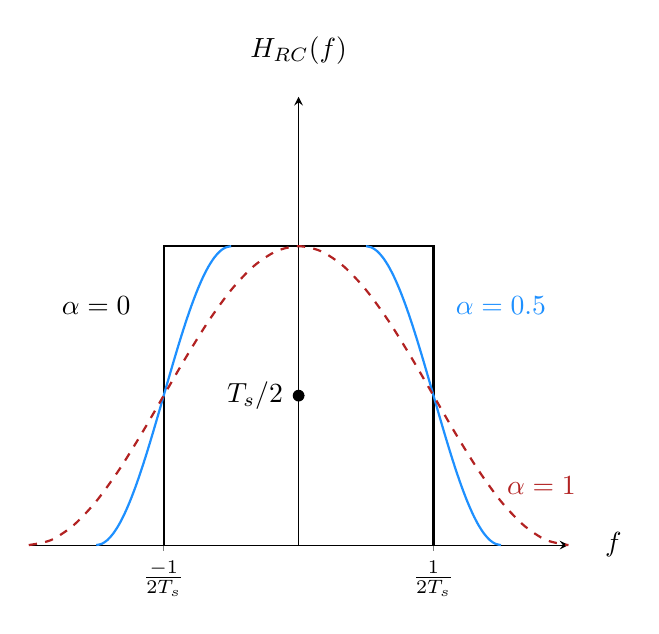
\begin{tikzpicture}
        \begin{axis}[
                axis lines=middle,
                xlabel={$f$},
                ylabel={$H_{RC}(f)$},
                xtick={-0.5, 0.5},
                xticklabels={$\frac{-1}{2T_s}$, $\frac{1}{2T_s}$},
                ytick={0.5},
                yticklabels={$T_s/2$},
                ymin=0, ymax=1.5,
                xmin=-1, xmax=1,
                every axis x label/.style={at={(ticklabel* cs:1.05)}, anchor=west,},
                every axis y label/.style={at={(ticklabel* cs:1.05)}, anchor=south,},
                xmajorgrids=false,
                ymajorgrids=false,
                clip=false,
                no markers,
            ]

            % Draw the ideal filter response (black box)
            \draw [thick] (axis cs:-0.5,0) -- (axis cs:-0.5,1) -- (axis cs:0.5,1) -- (axis cs:0.5,0);

            % Draw the realistic filter response for alpha = 0.5 (blue line)
            % \addplot [myblue, thick, smooth, domain=-1:1] {0.5+0.5*cos(deg(pi*x))};
            \addplot [myblue, thick, smooth, domain=-0.75:0.-0.25] {0.5 * (1 + cos(deg(pi*(abs(x)-0.25)/0.5)))};
            \addplot [myblue, thick, smooth, domain=0.25:0.75] {0.5 * (1 + cos(deg(pi*(abs(x)-0.25)/0.5)))};


            % Draw the realistic filter response for alpha = 1 (red dashed line)
            \addplot [myred, thick, dashed, smooth, domain=-1:1] {0.5-0.5*sin(deg(pi*(abs(x)-0.5))};

            % Add annotations for alpha values
            \node[myblue] at (axis cs:0.75,0.8) {$\alpha=0.5$};
            \node at (axis cs:-0.75,0.8) {$\alpha=0$};
            \node[myred] at (axis cs:0.9,0.2) {$\alpha=1$};

            % Add black dot at intersection
            \node[circle,fill,inner sep=1.5pt] at (axis cs:0,0.5) {};

        \end{axis}
    \end{tikzpicture}
\end{center}
\subsection*{Propriet\`a}
\begin{enumerate}
    \item Quando \( \alpha = 0 \) il coseno rialzato coincide con la funzione di trasferimento rettangolare
    \item La banda \( B_H \) \`e direttamente ottenibile da \( B_H = \frac{1+\alpha}{2T_S} \)
\end{enumerate}

La \( h_{RC}(t) \) \`e calcolabile in forma chiusa:

\[ h_{RC}(t) = \sin\left(\frac{t}{T_S}\right) \frac{\cos\left(\frac{\alpha \pi t}{T_S}\right)}{\left(1- \frac{2\alpha t}{T_S}\right)^2}  \]

\[ h_{RC}(kT_S) = \delta[k] \]

\begin{itemize}
    \item Soddisfa il criterio di Nyquist nel tempo, per cui garantisce l'assenza di ISI
    \item Decresce per \( t \rightarrow \infty \) come \( \frac{1}{|t|^3} \) per \( \alpha > 0 \) quindi molto pi\`u velocemente del caso \( \alpha = 0 \) (rettangolare)
\end{itemize}




\subsection*{Eccesso di banda e efficienza spettrale dei sistemi \( M-PAM \) con coseno rialzato}

Dato:
\[ p(t) \otimes c(t) \otimes h_R(t) = h_{RC}(t) \]
dove \( \otimes \) indica la convoluzione, $p(t)$ il sagomatore in trasmissione, $c(t)$ la risposta impulsiva del canale , $h_R(t)$ il filtro in ricezione e \( h_{RC}(t) \) la risposta impulsiva del filtro a coseno rialzato, l'efficienza spettrale del canale di comunicazione numerico è:
\[ \eta_{B} = \frac{\log_2M}{B_T T_s} = \frac{\log_2M}{B_H T_s} = \frac{\log_2M}{ T_s} \frac{2T_s}{1+\alpha} = \frac{2\log_2M}{1+\alpha}\]

Considerazioni:
\begin{itemize}
    \item L'efficienza spettrale, a parità di \( M \), decresce al crescere del coefficiente di roll-off (\( \alpha \)).
    \item La robustezza del sistema di comunicazione numerico all'ISI aumenta al crescere di \( \alpha \).
\end{itemize}

C'è quindi un trade-off tra robustezza all'ISI e efficenza spettrale, e i valori ottimali si trovano in corrispondenza di \( \alpha \simeq 0.4 \) .

\[ \text{Eccesso di banda richiesto dall'adozione del coseno rialzato:} \]
\[ \Delta B_{H} = B_{H} - \frac{1}{2T_s} = \frac{\alpha}{2T_s} \]



\subsection*{Prestazioni di un sistema di comunicazione numerico in banda base in presenza di rumore}

\paragraph*{Capacità di canale}

La capacità \( C \) di un canale di comunicazione è definita come il massimo valore che può assumere il tasso binario di segnalazione \( R_b = \frac{1}{T_b} \) al variare di tutte le possibili coppie modulatore/demodulatore, sotto il vincolo che la probabilità di errore sia esattamente nulla.


\[
    \begin{cases}
        C \coloneqq \max_{\{R_b\}} \\
        P_E(b) = P\{\hat{b}[n] \neq b[n]\} = 0
    \end{cases}
\]

La capacità di canale \( C \) si misura in bit/s ed è un numero non-negativo. Ovviamente, più è grande la capacità del canale e migliori sono le sue prestazioni.

\paragraph*{Capacità di canale con rumore gaussiano bianco additivo (AWGN)}

\begin{center}
    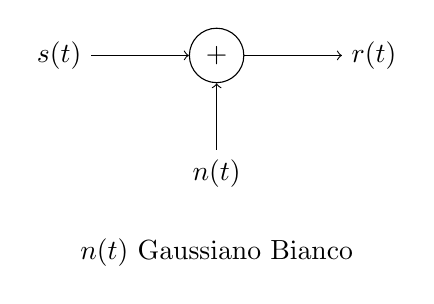
\begin{tikzpicture}
        \node (s) at (0,0) {\(s(t)\)};
        \node[draw, circle] (plus) at (2,0) {\(+\)};
        \node (n) at (2,-1.5) {\(n(t)\)};
        \node (r) at (4,0) {\(r(t)\)};

        \draw[->] (s) -- (plus);
        \draw[->] (n) -- (plus);
        \draw[->] (plus) -- (r);
        \node[below of=n, node distance=1cm] {\(n(t)\) Gaussiano Bianco};
    \end{tikzpicture}
\end{center}

In questo caso la capacità di canale può essere espressa in forma chiusa ed è in dipendenza dei parametri caratteristici del segnale trasmesso e del rumore.

\[
    C = B_T \log_2 \left( 1 + \frac{P_s}{N_0 B_T} \right) \quad \text{(Shannon)}
\]

Dove:
\begin{itemize}
    \item \( B_T \) = banda del segnale \( s(t) \)
    \item \( P_s \) = potenza media di \( s(t) \)
    \item \( \frac{N_0}{2} \) = DSP del rumore \( n(t) \) (costante essendo bianco)
\end{itemize}

Considerazioni:

\begin{enumerate}
    \item Fissato \( B_T \)
          \begin{align*}
              \lim_{\frac{P_s}{N_0} \to \infty} C & = 0       \\
              \lim_{\frac{P_s}{N_0} \to \infty} C & = +\infty
          \end{align*}

    \item Fissato \( \frac{P_s}{N_0} \)
          \begin{align*}
              \lim_{B_T \to \infty} C & = 0                              \\
              \lim_{B_T \to \infty} C & = \log_2 e \cdot \frac{P_s}{N_0}
          \end{align*}

    \item Riscrivendo la formula di Shannon utilizzando \( P_s = E_b R_b \)
          \[
              \frac{C}{B_T} = \log_2 \left( 1 + \frac{E_b}{N_0} \cdot \frac{R_b}{B_T} \right)
          \]
          Dove:
          \begin{itemize}
              \item \( E_b \) = energia per bit
              \item \( R_b \leq C \) (data la definizione di \( C \) come valore massimo di \( R_b \))
          \end{itemize}
\end{enumerate}

\paragraph*{Sistema di comunicazione numerico ideale}
Un sistema di comunicazione numerico è detto ideale se soddisfa le seguenti condizioni:
\begin{enumerate}
    \item \( R_b = C \)
    \item \( P_E(b) = 0 \)
\end{enumerate}

In queste condizioni è possibile mettere in relazione l'efficienza spettrale con il rapporto \( \frac{E_b}{N_0} \) (legato all
efficienza in potenza)

\[
    \eta_B = \log_2 \left( 1 + \frac{E_b}{N_0} \eta_B  \right) \quad \text{soggetto a} \quad  \eta_B = \frac{R_b}{B_T} = \frac{C}{B_T}
\]

\[
    \Rightarrow \frac{E_b}{N_0} = \frac{2^{\eta_B} - 1}{\eta_B} \quad \text{con} \quad \eta_B \geq 0
\]


\paragraph*{Considerazioni}

\begin{enumerate}
    \item
          $\lim_{\eta_B \to +\infty} \frac{2^{\eta_B } - 1}{\eta_B } = +\infty$


    \item $\lim_{\eta_B \to +\infty} \frac{2^{\eta_B } - 1}{\eta_B } = \ln{2} \quad (-1.6 \, \text{dB})$

\end{enumerate}


\subsection*{Ricezione ottima in presenza di rumore bianco}

Per il momento consideriamo solo gli effetti relativi al rumore.

\begin{center}
    \begin{tikzpicture}[
            block/.style={rectangle, draw, minimum height=1cm, minimum width=2cm},
            node distance=3cm and 3cm,
            auto
        ]

        \node[block] (filter) {$h_R(t)$};
        \node[left=of filter] (channel) {};
        \node[right=of filter] (sampler) {};
        \draw[->] ([xshift=-3cm]filter.west) -- (filter.west) node[midway,above] {$r(t)=s(t)+n(t) \quad$};


        \draw ([xshift=0]filter.east) -- ([xshift=3.5cm]filter.east) node[midway,above] {$y(t)=s_u(t)+n_u(t)$};
        \draw ([xshift=3.5cm]filter.east) -- ([xshift=4cm,yshift=0.5cm]filter.east) node[midway,below, yshift=-0.2cm] {$T_s$};

        \draw[->] ([xshift=4cm,yshift=0cm]filter.east) -- ++(1.5cm,0) node[midway,above] {$y[k]$};
    \end{tikzpicture}
\end{center}
Dove \( s(t) \) è un segnale di forma nota e \( n(t) \) è un rumore additivo bianco

\[
    s_u(t) = s(t) \ast h_R(t), \quad n_u(t) = n(t) \ast h_R(t)
\]

\[
    y(T_s) = s_u(T_s) + n_u(T_s)
\]

Si definisce il rapporto segnale-rumore in uscita al filtro \( h_R(t) \) all'istante \( t = T_s \) come

\[
    SNR \coloneqq \frac{s_u^2(T_s)}{E[n_u^2(T_s)]}
\]

Si definisce ricevitore ottimo il filtro \( h_R(t) \) che massimizza l'SNR in uscita al filtro.

Nel caso di rumore bianco in ingresso il filtro ottimo prende il nome di \textbf{filtro adattato}

Problema:
\begin{enumerate}
    \item Derivare il filtro \( h_R(t) \) che massimizza l'SNR all'uscita.
    \item Determinare il valore massimo dell'SNR all'uscita.
\end{enumerate}


\paragraph*{Derivazione del filtro adattato}

L'SNR viene espressa come:
\[
    \text{SNR} = \frac{s_u^2(T_s)}{E[n_u^2(T_s)]}
\]

Calcoliamo i termini al numeratore e al denominatore della SNR.
\[
    s_u^2(T_s) = \left( \int_{-\infty}^{+\infty} s(\tau) h_R(T_s - \tau) d\tau \right)^2 = \left( \int_{-\infty}^{+\infty} S(f) H_R(f) e^{j2\pi fT_s} df \right)^2
\]

E l'energia del rumore all'uscita del filtro ricevitore sarà:
\[
    E[n_u^2(T_s)] = R_{n_u}(0)
\]

Dove:
\[
    R_{n_u}(\tau) = R_n(\tau) \ast h_R(\tau) \ast h_R(-\tau)
\]

E quindi per la potenza del rumore:
\[
    S_{n_u}(f) = S_n(f) \left| H_r(f) \right|^2 = \frac{N_0}{2} \left| H_R(f) \right|^2
\]

\[
    R_{n_u}(0) = \int_{-\infty}^{+\infty} S_{n_u}(f) df
\]

Sostituendo otteniamo l'SNR in funzione della risposta in frequenza del filtro ricevitore \( h_R(f) \):
\[
    \text{SNR} = \frac{\left( \int_{-\infty}^{+\infty} S(f) H_R(f) e^{j2\pi fT_s} df \right)^2}{\frac{N_0}{2} \int_{-\infty}^{+\infty} \left| H_R(f) \right|^2 df} = \frac{2}{N_0 E_{h_R}} \left( \int_{-\infty}^{+\infty} S(f) H_R(f) e^{j2\pi fT_s} df \right)^2
\]

Utilizzando la disuguaglianza di Schwarz si può dimostrare che $\int_{-\infty}^{+\infty} S(f) H_R(f) e^{j2\pi fT_s} df$ raggiunge il massimo valore quando:
\[
    H_R(f) e^{j2\pi fT_s} = S^*(f)
\]

Quindi:
\[
    H_R(f) = S^*(f) e^{-j2\pi fT_s}
\]

\[
    \boxed{h_R(t) = s(T_s - t)}
\]

Dalla espressione della risposta impulsiva \( h_R(t) \) si deduce il nome di \textbf{filtro adattato}, in quanto la sua risposta impulsiva è adattata al segnale in ingresso al filtro stesso.



Studiando il modulo della risposta in frequenza \( H_R(f) \) si deduce che il filtro tende ad amplificare le componenti frequenziali dove è presente il segnale e ad attenuare (o eliminare) le componenti frequenziali dove il contributo di segnale è scarso (o addirittura assente).

\[
    \left| H_R(f) \right| = \left| S(f) \right|
\]

La simbologia per indicare un filtro adattato è \( h_{FA}(t) \) o \( H_{FA}(f) \).

Esempio:

% Drawing the example signals using TikZ
\begin{tikzpicture}
    \draw[->] (-1,0) -- (5,0) node[right] {\(t\)};
    \draw[->] (0,-1) -- (0,2) node[above] {\(s(t)\)};
    \draw[dashed] (0,1) -- (1,1);
    \node at (0,1) [left] {\(1\)};
    \draw (0,0) -- (1,1) -- (1,0);
    \node at (1,0) [below] {\(T_s\)};
    \draw[->] (6,0) -- (12,0) node[right] {\(t\)};
    \draw[->] (7,-1) -- (7,2) node[above] {\(h_{FA}(t)\)};
    \draw (7,1) -- (8,0);
    \node at (8,0) [below] {\(T_s\)};
\end{tikzpicture}

Calcolo del \( SNR_{max} \)

Il valore del \( SNR_{max} \) si ottiene per definizione quando si utilizza il \( FA \).

\[
    SNR = \frac{2}{N_0 E_s} \cdot E_s^2 = \frac{2E_s}{N_0}
\]

Da notare che:

\begin{itemize}
    \item Il \( SNR \) non dipende dalla forma del segnale, ma solo dalla sua energia. Questo da spazio alla progettazione della forma del segnale indipendentemente dai risultati in termini di \( SNR \).
    \item Il massimo del \( SNR \) si ottiene per qualunque \( h_{FA}(t) = k \cdot s(T_s-t) \) con \( k \in \mathbb{R} \), infatti basta calcolare il $SNR$:
          \[ SNR = \frac{2}{N_0K^2 E_s} \cdot K^2 E_s^2 = \frac{2 E_s}{N_0} \]
\end{itemize}

Quindi, fattori di amplificazione e/o attenuazione non cambiano il risultato. Questo è abbastanza intuitivo in quanto un fattore costante di amplificazione opera allo stesso modo sul segnale utile e sul rumore per cui nel rapporto i contributi si elidono.

\paragraph*{Schema del ricevitore con filtro adattato}

Consideriamo la trasmissione di un simbolo:

\begin{center}
    \begin{tikzpicture}[
            block/.style={rectangle, draw, minimum height=1cm, minimum width=2.5cm},
            node distance=1cm and 2cm,
            auto
        ]




        \node[block] (filter) {$h_{FA}(t)$};
        %\node[left=of filter] (channel) {};
        \node[right=of filter] (sampler) {};




        \node (s) at (-5,0) {\(s(t)\)};
        \node[draw, circle] (plus) at (-3,0) {\(+\)};
        \node (n) at (-3,-1.5) {\(n(t)\)};

        \draw[->] (s) -- (plus);
        \draw[->] (n) -- (plus);
        %\draw[->] (plus) -- (channel);

        \draw[->] (plus) -- (filter) node[midway,above] {$r(t)$};

        \draw ([xshift=0]filter.east) -- ([xshift=1cm]filter.east) node[midway,above] {$y(t)$};
        \draw ([xshift=1cm]filter.east) -- ([xshift=1.5cm,yshift=0.5cm]filter.east) node[midway,below, yshift=-0.2cm] {$kT_s$};

        \draw[->] ([xshift=1.5cm,yshift=0cm]filter.east) -- ++(1.5cm,0) node[midway,above] {$y[k]$};


    \end{tikzpicture}
\end{center}

\[ s(t) = \alpha \cdot p(t-nTs) \]
\[ h_{FA}(t) = k \cdot p(T_s - t) \]
\[ y(t) = s_u(t) + n_u(t) \]

Caratteristiche di \( s_u(t) \) e \( n_u(t) \):

\[ s_u(t) = s_u(t) \ast h_{FA}(t) = k \cdot \alpha \cdot p(t) \ast p(T_s - t) \]
\[ = k \cdot \alpha \int_{-\infty}^{\infty} p(\tau) p(\tau - (t - T_s)) d\tau = k \cdot \alpha \cdot C_p (t - T_s) \]
\[ C_p(t) = \int_{-\infty}^{\infty} P(\tau) P(\tau - t) d\tau \quad \text{(Autocorrelazione dell'impulso sagomatore)}
\]

\textbf{Esempio:}\\
La funzione rettangolare:
\[ s(t) = \text{rect}\left(\frac{t - \frac{T_s}{2}}{T_s}\right) \]

La risposta unitaria:
\[ s_u(t) = C_s(t - T_s) = T_s\cdot \left( 1 - \frac{\left| t - T_s \right|}{T_s} \right) \text{rect}\left(\frac{t - T_s}{2T_s}\right) \]
\noindent
\begin{minipage}{.5\textwidth}
    \centering

    % Diagrammi usando TikZ
    \begin{tikzpicture}
        \begin{axis}[
                axis lines = middle,
                xlabel = \( t \),
                ylabel = \( s(t) \),
                xtick = {1},
                xticklabels={$T_s$},
                ytick = {1},
                ymin = 0, ymax = 3.5,
                xmin = 0, xmax = 2.5,
                every axis x label/.style={at={(current axis.right of origin)},anchor=west},
                every axis y label/.style={at={(current axis.above origin)},anchor=south}
            ]
            \addplot+[const plot, no marks, thick] coordinates {(0,1) (1,1) (1,0)};
        \end{axis}
    \end{tikzpicture}
\end{minipage}%
\begin{minipage}{.5\textwidth}
    \centering
    \begin{tikzpicture}
        \begin{axis}[
                axis lines = middle,
                xlabel = \( t \),
                ylabel = \( s_u(t) \),
                xtick = {1, 2},
                xticklabels={$T_s$, $2T_s$},
                ytick = {1},
                yticklabels={$T_s$},
                ymin = 0, ymax = 2.5,
                xmin = 0, xmax = 2.5,
                every axis x label/.style={at={(current axis.right of origin)},anchor=west},
                every axis y label/.style={at={(current axis.above origin)},anchor=south}
            ]
            \draw[dashed] (0, 1) -- (1, 1) -- (1,0);
            \addplot+[sharp plot, no marks, thick] coordinates {(0,0) (1,1) (2,0)};
        \end{axis}
    \end{tikzpicture}
    \\
\end{minipage}


\[ n_u(t) = n(t) \ast h_{FA}(t) \]
\[ n(t) = \text{rumore bianco Gaussiano additivo (AWGN)} \]
\[ E[n(t)] = 0 \]
\[ R_n(\tau) = \sigma_n^2 \delta(\tau) = \frac{N_0}{2} \delta(\tau) \]
\[ n(\overline{t}) = \text{variabile aleatoria con densità di probabilità } f_N(n) = \frac{1}{\sqrt{2\pi\sigma_n^2}} e^{-\frac{n^2}{2\sigma_n^2}} = \frac{1}{\sqrt{N_0}} e^{-\frac{n^2}{N_0}} \]
Essendo il filtro in ricezione un filtro lineare e stazionario, \( n_u(t) \) è un rumore Gaussiano, additivo e stazionario.
\[ E[n_u(t)] = 0 \]
\[ R_{n_u}(\tau) = R_n(\tau) \ast h_{FA}(\tau) \ast h_{FA}(-\tau) = \frac{N_0}{2} C_{h_{FA}}(\tau)  \]
\[
    C_{h_{FA}}(\tau) = \text{autocorrelazione di } h_{FA}(t)
\]
\[ S_{n_u}(f) = \frac{N_0}{2} |H_{FA}(f)|^2 \]
\[ P_{n_u} = \frac{N_0}{2} E_{H_{FA}} = \frac{N_0}{2} E_p k^2 \]

È importante capire se i campioni di rumore sono tutti loro correlati o meno.
\[
    E[n_u[k]n_u[n]] = 0 \quad \forall k \neq n \quad \text{(incorrelazione)}
\]
N.B. la si può scrivere così poiché
\(E[n_u[k]] = 0\)

Questo vuol dire che
\[
    R_{n_u}[kT_s] = 0 \quad \forall k \neq 0
\]

\[
    R_{n_u}[nT_s] = \frac{N_0}{2} C_p[kT_s] = 0 \Rightarrow C_p[kT_s] = 0
\]


Dobbiamo ricordare che il segnale utile in ingresso al filtro adattato è ottenuto tramite il modulatore in trasmissione per cui è la funzione \( p(t) \) che determina la sagoma (forma) del segnale \( s(t) \).

\begin{enumerate}
    \item Impulso rettangolare
          \[
              p(t) = \text{rect}\left(\frac{t-T_s/2}{T_s}\right)
          \]

          \[
              C_p(\tau) = T_s \left(1 - \frac{|\tau|}{T_s}\right) \text{rect}\left(\frac{\tau}{2T_s}\right)
          \]

          \[
              R_{n_u}(\tau) = k \frac{N_0}{2} C_p(\tau)
          \]

          \[
              R_{n_u}(nT_s) =
              \begin{cases}
                  \frac{k^2 N_0 T_s}{2} & \text{se } k = 0    \\
                  0                     & \text{se } k \neq 0
              \end{cases}
              \Rightarrow
              \text{campioni di rumore incorrelati} \Rightarrow \text{indipendenti (Gaussiani)}
          \]
          \begin{center}
              \begin{tikzpicture}
                  \draw[->] (-3.5,0) -- (3.5,0) node[right] {$\tau$};
                  \draw[->] (0,-0.5) -- (0,2) node[above] {$C_p(\tau)$};
                  \draw[scale=1,domain=-1.5:1.5,smooth,variable=\x] plot ({\x},{1.5-abs(\x)});
                  \draw (1.5,0.1) -- (1.5,-0.1) node[below] {$T_s$};
                  \draw (-1.5,0.1) -- (-1.5,-0.1) node[below] {$-T_s$};
                  \draw (0.1,1.5) -- (-0.1,1.5) node[left] {$T_s$};
              \end{tikzpicture}

          \end{center}
    \item Impulso a radice di coseno rialzato
          \[
              P(f) = \sqrt{H_{RC}(f)}
          \]

          \begin{align*}
              S_{n_u}(f)    & = k^2 \frac{N_0}{2} |P(f)|^2 = k^2 \frac{N_0}{2} H_{RC}(f) \\
              R_{n_u}(\tau) & = k^2 \frac{N_0}{2} h_{RC}(\tau)                           \\
              R_{n_u}(nT_s) & = \begin{cases}
                                    \frac{k}{2} N_0, & k = 0    \\
                                    0,               & k \neq 0
                                \end{cases} \quad
              \text{N.B. la $h_{RC}(\tau)$ ha la sinc che si annulla in multipli di $T_s$.}
          \end{align*}

\end{enumerate}


\paragraph{SNR per bit all'ingresso del ricevitore}

Il SNR per bit è un parametro utile per determinare le prestazioni di una ricevitore in quanto tiene in considerazione quantità energetiche sia del segnale utile che del rumore
\[
    SNR_b = \frac{E_b}{N_0}
\]
\[
    E_b \coloneqq P_s T_b = E\left[x^2[k]\right]T_b \quad \text{Energia per bit} \]
\[
    \frac{N_0}{2} = S_n(f)
    \Rightarrow SNR_b = \frac{E\left[ x[k]\right]}{N_0 R_b}, \quad R_b = \frac{1}{T_b}
\]

\paragraph{Decisore ottimo e criterio della massimo verosimiglianza}

Il decisore deve mappare i campioni $y[k]$ in simboli dell'alfabeto. I campioni $y[k]$ sono statisticamente indipendenti l'uno dall'altro. Questo è dimostrato dal fatto che:

\[
    y[k] = s_u[k] + n_u[k]
    \quad
    \text{dove } s_u(k) \text{ e } n_u(k) \text{ sono indipendenti}
\]


%\draw[->] (source) -- (encoder) node[midway,above] {$b[n]$}  node[midway,below] {$T_b$};
\begin{center}
    \begin{tikzpicture}[
            block/.style={rectangle, draw, minimum height=1cm, minimum width=2.5cm},
            node distance=1cm and 2cm,
            auto
        ]
        \node[block] (filter) {Decisore};
        \node[left=of filter] (channel) {};
        \node[right=of filter] (sampler) {};

        \draw[->] (channel) -- (filter) node[midway,above] {$y[k]$}  node[midway,below] {$T_b$};
        \draw[->] (filter) -- (sampler) node[midway,above] {$\hat{x}[k]$}  node[midway,below] {$T_b$};
    \end{tikzpicture}
\end{center}

Quindi si può concludere che $\hat{x}[k] \in A_s $ può essere deciso in base alla sola conoscenza di $y[k]$. Questa decisione si dice di tipo "ad un sol colpo" (one-shot detector).

\paragraph{Decisione a minima probabilità di errore}

\begin{itemize}
    \item Probabilità di errore sul simbolo
          \(
          P_E(M) \coloneqq P\{\hat{x}[k] \neq x[k]\}
          \)
    \item
          Criterio di ottimalità: minimizzazione della $P_E(M)$

\end{itemize}

Derivazione del decisore ottimo:
\[
    x \coloneqq \hat{x}[k], \quad y \coloneqq y[k], \quad n_u \coloneqq n_u[k], \quad \hat{x} = \hat{x}[k]
\]

\paragraph{Criterio a massima probabilità a posteriori e minima probabilità di errore}
Con
MAP si intende l'acronmo di Maximum A-posteriori Probability
\[
    \hat{x} = \arg\max_{i=1,\ldots,M} P(x=\alpha_i|y)
\]

Viene associato ad un osservato $y$ il simbolo dell'alfabeto $\hat{x}$ tale che sia massima la probabilità a posteriori (condizionata) che quel simbolo sia stato trasmesso.

Se il decisore adotta il criterio MAP allora la probabilità di errore sul simbolo è minima.


\paragraph{Dimostrazione}

Definiamo
\(
R(i) \coloneqq \left\{ y \in \mathbb{R} : \hat{x} = \alpha_i \right\}, \quad i = 1,\ldots,M
\)
come la "zona di decisione" del simbolo $\alpha_i$, ovvero l'insieme dei valori di $y$ per cui si decide per il simbolo $\alpha_i$.

\[
    P\{x = \alpha_i | y\} = \frac{f_Y(y | \hat{x} = \alpha_i) P\{x = \alpha_i\}}{f_Y(y)} \quad (\text{Bayes})
\]

\[
    P_E(M) = P\{\hat{x} \neq x\} = 1 - P\{\hat{x} = x\} = 1 - \sum_{i=1}^M P\{\hat{x} = \alpha_i, x = \alpha_i\}
\]

\[
    = 1 - \sum_{i=1}^M P\{\hat{x} = \alpha_i | x = \alpha_i\} P\{x = \alpha_i\} =
\]

\[
    = 1 - \sum_{i=1}^M P\{x = \alpha_i\} P\{y \in R(i) | x = \alpha_i\}
\]

\[
    = 1 - \sum_{i=1}^M P\{x = \alpha_i\} \int_{y \in R(i)} f_Y(y | x = \alpha_i) dy
\]

\[
    = 1 - \sum_{i=1}^M \int_{y \in R(i)} P\{x = \alpha_i\} f_Y(y | x = \alpha_i) dy
\]

\[
    = 1 - \sum_{i=1}^M \int_{y \in R(i)} f_Y(y) P\{x = \alpha_i | y\} dy
\]

Per minimizzare la $P_E(M)$ devo scegliere le $R(i)$ in modo tale che osservato $y$ sia massima la probabilità a posteriori relativa al simbolo $i$-esimo.

Si osserva che se le probabilità a priori sono identiche
\[
    P\{x = a_i\} = \frac{1}{M}, \quad i=1,\ldots,M
\]
allora, dato che $f_Y(y)$ non dipende da $i$:
\[
    \hat{x} = \arg \max_{i=1,\ldots,M} \left\{ \frac{1}{M} \frac{f_Y(y | x = \alpha_i)}{f_Y(y)} \right\} = \arg \max_{i=1,\ldots,M} f_Y(y | x = \alpha_i)
\]


La funzione $f_Y(y|x=\alpha_i)$ viene detta anche \textbf{funzione di verosimiglianza}

In pratica il criterio di minima probabilità di errore (o massima probabilità a posteriori) coincide con il criterio di massima verosimiglianza quando le probabilità a priori $P\{x=\alpha_i\}$ sono identiche.
Nel caso di AGWN
\[
    y = s_u + n_u = \alpha_i + n_u, \quad n_u \in \mathcal{N}(0,\sigma_{n_u}^2)
\]
\[
    f_Y(y|x = \alpha_i) = f_{n_u}(y - \alpha_i)
\]
\[
    = \frac{1}{\sqrt{2\pi\sigma_{n_u}^2}} e^{-\frac{(y-\alpha_i)^2}{2\sigma_{n_u}^2}}
\]

\[
    \hat{x} = \underset{i=1,\ldots,M}{\mathrm{argmax}} \frac{1}{\sqrt{2\pi\sigma_{n_u}^2}} e^{-\frac{(y-\alpha_i)^2}{2\sigma_{n_u}^2}} = \underset{i=1,\ldots,M}{\mathrm{argmin}}  (y - \alpha_i)^2
\]

\[
    \boxed{
        \hat{x} = \underset{i=1,\ldots,M}{\mathrm{argmin}} \{ |y-\alpha_i| \}
    } \quad \text{(minimo della distanza euclidea)}
\]


Il decisore ottimo coincide con la scelta del simbolo a distanza euclidea minima dall'osservato.

Le zone di decisione sono quindi stabilite dalla regola di quantizzazione uniforme.

Questo significa che il decisore può essere realizzato con un quantizzatore uniforme.


\paragraph{Ricevitore ottimo per un sistema di comunicazione PAM}

Per un sistema di comunicazione PAM con simboli equiprobabili, il ricevitore ottimo secondo il criterio a minima probabilità di errore è il seguente:

\begin{center}
    \begin{tikzpicture}[
            block/.style={rectangle, draw, minimum height=1cm, minimum width=2.5cm},
            node distance=3cm and 3cm,
            auto
        ]

        \node[block] (filter) {$p(T_s - t)$};
        \node[left=of filter] (channel) {};
        \node[right=of filter] (sampler) {};
        \node[block, right=of filter](quantizzatore) {Quantizzatore uniforme M livelli};

        \draw[->] (channel) -- (filter) node[midway,above] {$r(t)$};

        \draw ([xshift=0]filter.east) -- ([xshift=1cm]filter.east) node[midway,above] {$y(t)$};
        \draw ([xshift=1cm]filter.east) -- ([xshift=1.5cm,yshift=0.5cm]filter.east) node[midway,below, yshift=-0.2cm] {$T_s$};

        \draw[->] ([xshift=1.5cm,yshift=0cm]filter.east) -- ++(quantizzatore) node[midway,above] {$y[k]$};

        \draw[->] (quantizzatore.east) -- ++(1.5cm,0) node[midway,above] {$\hat{x}[k]$};

    \end{tikzpicture}
\end{center}

\begin{figure}
    \centering
    \begin{center}
        \begin{tikzpicture}[scale=0.75]
            % Assi
            \draw[thick,->] (-6,0) -- (6,0) node[anchor=north west] {};
            \draw[thick,->] (0,-5) -- (0,5) node[anchor=south east] {};

            % Grafico a gradini
            \draw[ultra thick, red] (-4,-3) -- (-2,-3) -- (-2,-1) -- (0,-1) -- (0,1) -- (2,1) -- (2,3) -- (4,3);

            % Tacche e etichette sull'asse delle x
            \foreach \x in {-4,-2,2,4}
            \draw (\x cm,1pt) -- (\x cm,-3pt)
            node[anchor=north] {$\x$};


            % Linee tratteggiate
            \draw[dashed, red] (-4,0) -- (-4,-3);
            \draw[dashed, red] (-2,-1) -- (-2,0);

            \draw[dashed, red] (4,0) -- (4,3);
            \draw[dashed, red] (2,1) -- (2,0);
            \draw[dashed, red] (2,3) -- (0,3);
            \draw[dashed, red] (-2,-3) -- (0,-3);

            % Etichette
            \node at (0,1) [left] {$1$};
            \node at (0,-1) [right] {$-1$};
            \node at (0,3) [left] {$3$};
            \node at (0,-3) [right] {$-3$};
        \end{tikzpicture}
    \end{center}
    \caption*{Esempio di una 4-Pam, con quantizzatore uniforme a 4 livelli}
\end{figure}

\paragraph{Probabilità di errore di bit e di simbolo}

\[
    P_E(b) = P\{\hat{b}[k] \neq b[k]\} \quad \text{bit}
\]

\[
    P_E(M) = P\{\hat{x}[k] \neq x[k]\} \quad \text{simbolo}
\]

\[
    P_E(M) = P_E(b) \quad \text{solo quando l'alfabeto } A_s \text{ è composto da soli due simboli}
\]
Vale però sempre che:
\[
    \frac{P_E(M)}{\log_2 M} \leq P_E(b) \leq \frac{M/2}{M-1} P_E(M)
\]

\paragraph{Codifica di Gray}

Sia \( A_s = \{\alpha_1, \ldots, \alpha_M\} \) dove
\[
    \alpha_i = 2i - M - 1 \quad i = 1, \ldots, M
\]

La codifica di Gray associa stringhe di bit ai simboli dell'alfabeto in modo che le stringhe di bit relative a due simboli consecutivi differiscano al più per un bit.

Nel caso di SNR sufficientemente elevato \( (> 10 dB) \), l'evento errore consiste generalmente nel decidere per uno dei simboli dell'alfabeto adiacenti a quello trasmesso.

Utilizzando quindi la codifica di Gray e in condizioni di SNR elevato, un errore su un simbolo \( M-ario \) ogni \( N \) simboli  \( M-ari \) si traduce in un errore su una sola cifra binaria ogni \( N \) simboli \( M-ari \), cioè ogni \( N \log_2 M \) cifre binarie, quindi:

\[
    P_E(b) \approx \frac{P_E(M)}{\log_2 M}
\]


Esempi:

\begin{enumerate}
    \item 4-PAM
          \begin{itemize}
              \item $-3 \rightarrow 00$
              \item $-1 \rightarrow 01$
              \item $+1 \rightarrow 11$
              \item $+3 \rightarrow 10$
          \end{itemize}

    \item 8-PAM
          \begin{itemize}
              \item $-7 \rightarrow 000$
              \item $-5 \rightarrow 001$
              \item $-3 \rightarrow 011$
              \item $-1 \rightarrow 010$
              \item $+1 \rightarrow 110$
              \item $+3 \rightarrow 111$
              \item $+5 \rightarrow 101$
              \item $+7 \rightarrow 100$
          \end{itemize}
\end{enumerate}
\paragraph{Prestazioni di un M-PAM in presenza di rumore:}

\begin{center}
    \begin{tikzpicture}[
            block/.style={rectangle, draw, minimum height=1cm, minimum width=2.5cm},
            node distance=2.5cm and 2.5cm,
            auto
        ]




        \node[block] (filter) {$h_{FA}(t)$};
        \node[right=of filter] (sampler) {};
        \node[block, right=of filter](decisore) {Decisore};

        \node (s) at (-5,0) {\(s(t)\)};
        \node[draw, circle] (plus) at (-3,0) {\(+\)};
        \node (n) at (-3,-1.5) {\(n(t)\)};

        \draw[->] (s) -- (plus);
        \draw[->] (n) -- (plus);
        %\draw[->] (plus) -- (channel);

        \draw[->] (plus) -- (filter) node[midway,above] {$r(t)$};

        \draw ([xshift=0]filter.east) -- ([xshift=1cm]filter.east) node[midway,above] {$y(t)$};
        \draw ([xshift=1cm]filter.east) -- ([xshift=1.5cm,yshift=0.5cm]filter.east) node[midway,below, yshift=-0.2cm] {$T_s$};

        \draw[->] ([xshift=1.5cm,yshift=0cm]filter.east) -- (decisore) node[midway,above] {$y[k]$};
        \draw[->] (decisore.east) -- ++(1.5,0) node[midway,above] {$\hat{x}[k]$};

    \end{tikzpicture}
\end{center}

\[
    s(t) = \sum_{k=-\infty}^{\infty} x[k] P(t - kT_s)
\]

\[
    P_E(M) = \frac{M-1}{M} \text{erfc} \left( \sqrt{\frac{3\cdot SNR \cdot \log_2 M}{M^2-1}} \right)
\]

\begin{center}

    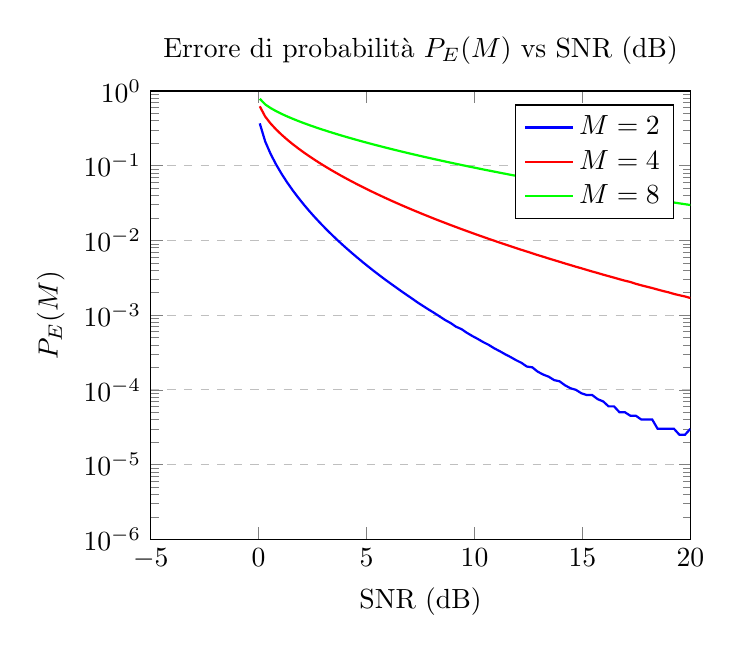
\begin{tikzpicture}
        \begin{axis}[
                title={Errore di probabilità $P_E(M)$ vs SNR (dB)},
                xlabel={SNR (dB)},
                ylabel={$P_E(M)$},
                xmin=-5, xmax=20,
                ymin=1e-6, ymax=1,
                ymode=log,
                legend pos=north east,
                ymajorgrids=true,
                grid style=dashed,
            ]

            % approximate erf(x) with tanh(1.2*x)
            \addplot[
                color=blue,
                mark=none,
                thick,
                domain=-5:20,
                samples=100,
            ] {0.5*(1-tanh(1.2*sqrt(x)))}; \addlegendentry{$M=2$}

            \addplot[
                color=red,
                mark=none,
                thick,
                domain=-5:20,
                samples=100,
            ] {0.75*(1-tanh(1.2*sqrt(2*x/5)))}; \addlegendentry{$M=4$}

            \addplot[
                color=green,
                mark=none,
                thick,
                domain=-5:20,
                samples=100,
            ] {0.875*(1-tanh(1.2*sqrt(x/7)))}; \addlegendentry{$M=8$}

        \end{axis}
    \end{tikzpicture}
\end{center}

Per SNR $> 10$ dB, utilizzando la codifica di Gray
\[
    P_E(b) \approx \frac{P_E(M)}{\log_2 M}
\]

Per una BPSK (2-PAM)
\[
    P_E(M) = P_E(b) = \frac{1}{2} \text{erfc}\left(\sqrt{\text{SNR}}\right)
\]

\paragraph{Dimostrazione}

Considerando le densità di probabilità $f_Y(y|x=1)$ e $f_Y(y|x=-1)$:

La probabilità di errore binario $P_E(b)$ è data dalla somma delle aree sotto le curve di $f_Y(y|x=1)$ e $f_Y(y|x=-1)$ dove queste si sovrappongono.



La densità di probabilità condizionata dato $x$ è:
\[
    P\{ \hat{x} = -1 | x = 1 \} = \int_{-\infty}^{\infty} f_Y(y | x = 1) \, dy
\]
\[
    f_Y(y | x = 1) = \frac{1}{\sqrt{2\pi \sigma_{n_u}^2}} \exp \left( -\frac{(y - h(0)x)^2}{2\sigma_{n_u}^2} \right) \quad \text{per} \quad x = 1
\]

Dopo il campionatore:
\[
    y[k] = x[k]\cdot h(0) + n_u[k]
\]

Dove la varianza del rumore è data da:
\[
    \sigma_{n_u}^2 = \frac{N_0}{2} E_{h_R} = \frac{N_0}{2} h(0)
\]

La densità spettrale di potenza del rumore bianco è:
\[
    S_w(f) = \frac{N_0}{2} \quad \Rightarrow \quad \text{DSP sul processo del rumore in ingresso è uguale in distribuzione } h_R(t)
\]

Il rapporto segnale-rumore (SNR) è:
\[
    SNR = \frac{h(0)^2}{\frac{N_0}{2} h(0)} = \frac{2 h(0)}{N_0}
\]

La probabilità condizionata dato $x$ è:
\[
    P\{ \hat{x} = -1 | x = 1 \} = 1 - Q\left( \frac{0 - h(0)}{\sqrt{\frac{N_0}{2} h(0)}} \right)
\]
\[
    = Q\left( \sqrt{\frac{2 h(0)}{N_0}} \right) = Q\left( \sqrt{SNR} \right) = \frac{1}{2} \text{erfc}\left( \sqrt{SNR} \right)
\]

Si può dimostrare per simmetria che:
\[
    P\{ \hat{x} = 1 | x = -1 \} = P\{ \hat{x} = -1 | x = 1 \} = \frac{1}{2} \text{erfc}\left( \sqrt{SNR} \right)
\]


Quindi:
\[
    P_E(b) = \frac{1}{2} \cdot \frac{1}{2} \text{erfc}\left( \frac{\sqrt{SNR}}{2} \right) + \frac{1}{2} \cdot \frac{1}{2} \text{erfc}\left( \frac{\sqrt{SNR}}{2} \right) = \frac{1}{2} \text{erfc}\left( \frac{\sqrt{SNR}}{2} \right)
\]

\paragraph{Presenza di ISI e rumore}

Il segnale ricevuto è:
\[
    y(t) = \sum_{k=-\infty}^{\infty} x[k] h(t - kT_s) + n_u(t)
\]

Dove:
\[
    h(t) = p(t) * c(t) * h_R(t)
\]
\[
    n_u(t) = n(t) * h_R(t)
\]

E il segnale al campionato è:
\[
    y[k] = x[k] \cdot h(0) + I[k] + n_u[k]
\]

Dove il termine di interferenza è dato da:
\[
    I[k] = \sum_{\substack{n=-\infty \\ n \neq k}}^{+\infty} x[n] h\left( (k-n)T_s \right)
\]

L'approccio da seguire è il seguente:
il filtro $h_R(t)$ deve essere allo stesso tempo quello che elimina l'ISI e che massimizza l'$SNR$. Questo problema può essere risolto progettando opportunamente $p(t)$ e $h_R(t)$.

\paragraph{Equalizzatore zero forcing}

Massimizza il SNR vincolando \( I[k] = 0 \) per ogni \( k \).  È un problema di massimizzazione vincolata per cui la soluzione non porta alla realizzazione del filtro adattato.

\begin{itemize}
    \item \( I[k] = 0 \) quando \( h(t) = h_{RC}(t) \), allora
          \[
              P(f) C(f) H_R(f) = H(f) = H_{RC}(f) e^{-j 2 \pi f T_s}
          \]
          per la causalità.

          Si pone quindi il problema di massimizzare il $SNR$ con il vincolo
          \[
              P(f) C(f) H_R(f) = H_{RC}(f) e^{-j 2 \pi f T_s}
          \]
\end{itemize}

Si può scrivere:
\[
    \left| P(f) \right| = \left| H_R(f) \right| = \sqrt{\frac{\left| H_{RC}(f) \right|}{\left| C(f) \right|}}
\]
\[
    \angle P(f) = \angle H_R(f) = - \pi f T_s - \frac{\angle C(f)}{2}
\]

N.B. Se \( C(f) = 1 \) (canale ideale) allora
\[
    P(f) = H_R(f) = \sqrt{H_{RC}(f)} e^{-j 2 \pi f T_s}
\]

Il valore di SNR in tal caso è:



\[
    SNR = \frac{E\left\{\left|X[k]\right|^2\right\} h^2(0)}{\frac{N_0}{2}
    \int_{-B_c}^{B_c} \frac{H_{RC}(f)}{C(f)}\, df }
\]

dove \( B_c \) è la banda del canale \( C(f) \), \( h(t) \) è la risposta all'impulso del canale ideale e $h(0)$ può essere visto come $
    \int_{-\infty}^{+\infty} H(f)\, df$.

\[
    E_s = P_s T_s = T_s \frac{M^2-1}{3}
\]

Se \( C(f) = 1 \) allora \( SNR = \frac{2 E_s}{N_0} \) e il filtro è adattato.

Il segnale ricevuto è:
\[
    r(t) = \sum_{k=-\infty}^{\infty} x[k] p(t - kT_s) + n(t)
\]
dove \( n(t) \) è il rumore bianco additivo gaussiano (AWGN).

La funzione di trasferimento del filtro ricevitore è:
\[
    h_{R}(f) = p (T_s - t)
\]
\[
    H_{R}(f) = P(f) e^{-j2\pi fT_s}
\]
\[
    H(f) = P^2(f) e^{-j2\pi fT_s} = H_{RC}(f) e^{-j2\pi fT_s}
\]

Riassumendo, il problema di eliminare l'ISI e massimizzare il SNR si risolve utilizzando il filtro sagomatore \( p(t) \) e quello di ricezione, \( h_R(t) \), realizzati con la radice di coseno rialzato.

Nel caso di canale ideale, la soluzione coincide con il filtro adattato.
